\chapter{基于子树划分的抽象语法树表征学习}
\label{chap:AST}
本章主要对本文提出的基于子树划分的抽象语法树表征学习方法进行详细介绍,首先介绍其基本思想,其次阐述其具体方法设计与实现,最后进行实验验证。
\section{研究动机}
本文针对现有存在的问题,

抽象语法树AST是源代码语法结构的一种抽象表现形式,以树的形式包含了源代码中的语法信息和语法结构。利用深度神经网络对抽象语法树进行建模得到其向量表示,根据该特征向量完成代码克隆检测任务,实现基于树的源代码表征。现有的方法主要分为两类:一类是将AST转换为完整的二叉树,另一类是将AST直接视作二叉树,这两种方法都会或多或少破坏源代码原有的语法结构,而且在转换的过程会增加AST的高度,AST树过高会导致梯度消失问题,可能会丢失长期上下文信息,削弱了神经模型捕捉更真实和复杂语义的能力。
\section{AST表征方法设计}

本节将介绍基于子树划分的抽象语法树表征学习方法设计与实现, 

\subsection{框架概述}
基于子树划分的抽象语法树表征学习:

\subsection{子树划分}
针对上述问题,本文将每个大型的AST分割成小语句树序列,并通过捕获语句的词法和句法知识将每一个语句树都编码成一个向量。
\subsection{抽象语法树表征学习}
在得到一个语句向量序列后,将语句向量序列输入Tree LSTM网络中生成代码片段的结构向量表示。与标准LSTM结构类似,Tree-LSTM神经网络中每个神经元都包括类似的输入门,输出门和隐层输出。不同的是Tree-LSTM单元中门向量和神经元状态的更新依赖于所有与之相关的子单元的状态,另外,Tree-LSTM拥有多个遗忘门,分别对应当前节点的每个子节点,因此 Tree-LSTM可以选择性地从子节点中获取信息,从而保存语义信息更加丰富的子节点的信息。通过Tree LSTM模型,本文能够学习到基于抽象语法树的结构向量,通过这种连续向量表现基于树的理解认知层次,获取程序的结构信息,创建更高抽象层次上的表示,从而提高后续代码克隆检测任务的精度。


\section{AST表征方法具体实现}
\label{sec:achieve}

在介绍具体实现之前,本节首先给出AST表征方法的输入:经过\ref{subsec:Preprocess}小节的代码预处理阶段,得到示例代码片段\ref{fig:code}中$C_{a},C_{b}$对应的抽象语法树,如图\ref{fig:astcode}所示。
\begin{figure}[htbp]
  \centering  %居中
  \subfigure[C语言代码片段$C_{a}$对应的AST]{   %第一张子图
      \centering    %子图居中
      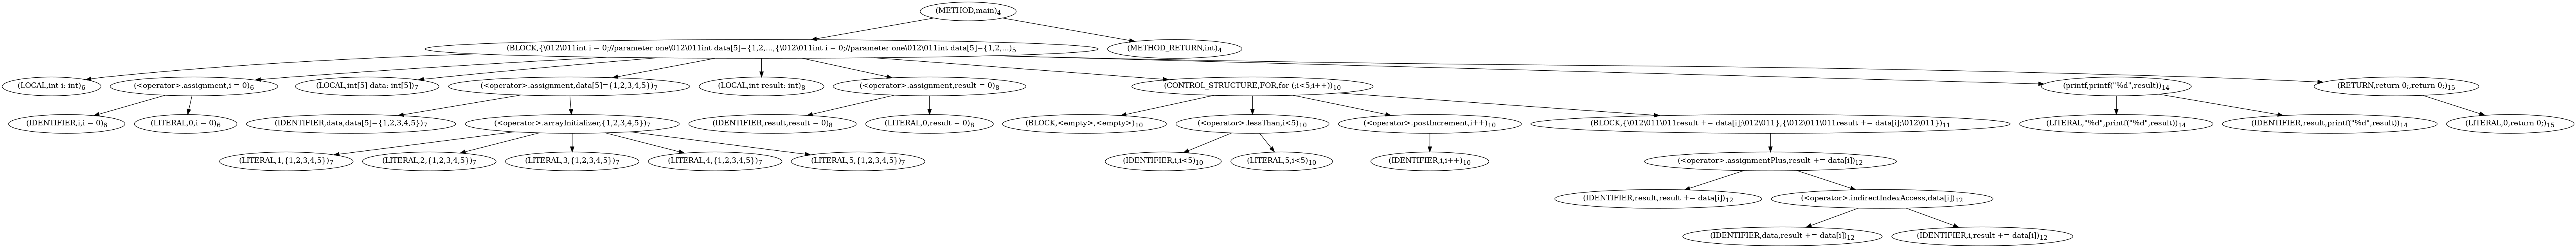
\includegraphics[width=0.85\textwidth]{figures/ast1}  
      \label{fig:ast1} %引用标签
  }
  \qquad
	%让图片换行,
  \subfigure[C语言代码片段$C_{b}$对应的AST]{ %第二张子图
      \centering    %子图居中
      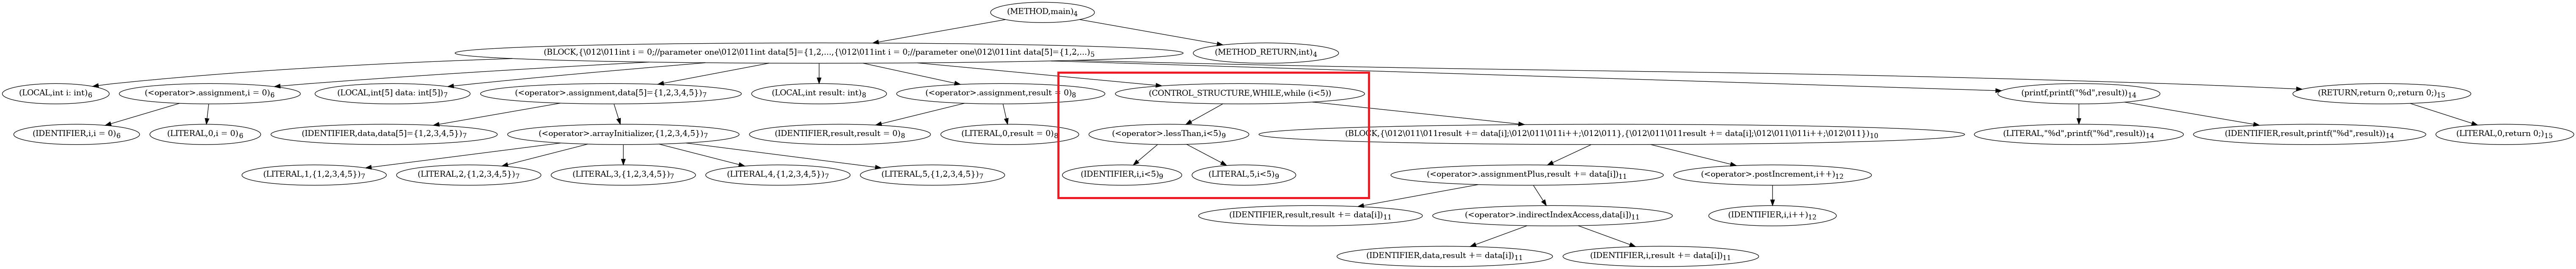
\includegraphics[width=0.85\textwidth]{figures/ast2}
      \label{fig:ast2} %引用标签
  }
  \caption{示例源代码对应的抽象语法树}    %大图名称
  \label{fig:astcode}    %图片引用标记
\end{figure}

\section{实验验证}
为了验证基于子树划分的抽象语法树表征学习方法的有效性,本文
\subsection{实验设计}
和3.3.1 相同
\subsection{抽象语法树子树划分消融实验结果}
消融对比实验:体现AST子树划分的有效性

基于AST的Tree-LSTM

基于AST的+子树划分的Tree-LSTM

\begin{table}
  \centering
  \caption{抽象语法树子树划分实验结果} %{tab:category}
  \begin{tabular*}{0.9\textwidth}{@{\extracolsep{\fill}}cccc}
  \toprule
    对比			&P		&R		&F1 \\
  \midrule
    基于AST的Tree-LSTM			&0.xx	&0.xx		&0.xx \\
    基于AST的+子树划分的Tree-LSTM			&0.xx		&0.xx		&0.xx \\
  \bottomrule
  \end{tabular*}
\end{table}

\section{本章小结}
本章



